% nastavenia prostredia
\documentclass[12pt,a4paper,titlepage,final]{report}
\usepackage[utf8]{inputenc}
\usepackage[T1, IL2]{fontenc}
\usepackage{graphicx}
\usepackage{epstopdf}
\usepackage{caption}
\usepackage[top=3cm, left=1cm, right=1cm, text={17cm, 24cm}, ignorefoot]{geometry}
\usepackage{color}
\usepackage{url}
\usepackage[bookmarksopen,colorlinks,plainpages=false,urlcolor=blue,unicode]{hyperref}

\begin{document}
	% define
	\def\authora{Michal Riša}
	\def\authorb{Pavel Macenauer}
	\def\emaila{xrisam01@stud.fit.vutbr.cz}
	\def\emailb{xmacen02@stud.fit.vutbr.cz}
	\def\docname{Firma2}
	\def\projname{Prvotná analýza a plán projektu}
	% titulna strana
	\begin{titlepage}
	\begin{center}
		
\includegraphics[height=5cm]{img/logo.eps}
	\end{center}
	\vfill
	\begin{center}
		\begin{Large}
			\docname\\
		\end{Large}
		\bigskip
		\begin{Huge}
			\projname\\
		\end{Huge}
	\end{center}
	\vfill
	\begin{center}
		\begin{large}
			\today
		\end{large}
	\end{center}
	\vfill
	\begin{flushleft}
		\begin{large}
			\begin{tabular}{lll}
				Autori: & \authora, & \url{\emaila} \\
				        & \authorb, & \url{\emailb} \\
				& & \\
				& Fakulta Informačných Technológií \\
				& Vysoké Učení Technické v Brně \\
			\end{tabular}
		\end{large}
	\end{flushleft}
\end{titlepage}

	% kapitoly
	\newpage
	\pagestyle{plain}
	\pagenumbering{arabic}
	\setcounter{page}{1}
	\setcounter{secnumdepth}{-1}
	

		% ----------- neformalni specifikace -----------

	\chapter{Analýza}
	
	\section{Neformální specifikace}
	Cílem projektu je navrhnout jednoduchý informační systém pro firmu organizující kursy orientované na programové vybavení počítačů, který ji umožní spravovat termíny kursů a zpracovávat přihlášky zákazníků.
	
	Kursy probíhají v pronajatých prostorech o různých kapacitách za vedení externích lektorů v různé termíny. Systém by tak měl zahrnovat možnost vypisovat kursy a k nim vytvořit prezentační (informační) stránku, ze které zákazník vyčte potřebné informace o kursu. Ke každému kurzu se budou vypisovat termíny a termínům přiřazovat cena, místo konání a lektor. Všechny tyto nastavení bude možno nadále i měnit.
	
	Součástí systému je i rozhraní, které umožní zákazníkům se přihlašovat na termíny. Každá přihláška bude mít jedinečný identifikátor, přes který bude možnost ji dohledat nebo spravovat. Po přihlášení se bude přihláška postupně zpracovávat pomocí daného protokolu mezi zákazníkem a zaměstnancem (přihlášení - potvrzení/odmítnutí - zaplacení - potvrzení platby).
	
	Systém by měl umožňovat správu uživatelů a změnu rolí jednotlivých uživatelů - lektor, zaměstnanec, administrátor. Tuto možnost bude mít pouze administrátor. Zákazníci nebudou mít uživatelské role a v systému budou evidování pomocí svých přihlášek.
	
	Zaměstnanec bude moci kdykoliv uzavřít nebo naopak otevřít přihlašování. I po zpracování přihlášky bude možnost měnit její stav, tzn. vyřadit ji z termínu nebo vrátit/zrušit platbu.
	
	Zákazníci budou mít možnost zažádat o vypsání konkrétního termínu nebo i kursu. Tato součást systému bude řešena jako komunikační kanál mezi žádajícím a zaměstnancem.
	
	Pro snadnou organizaci kurzů se budou jednotlivé termíny kursů zobrazovat v kalendáři, který si budou moci uživatelé systému zobrazit. Úroveň detailu kalendáře bude záviset na konkrétní roli uživatele.
	
	Systém bude implementován jako webová aplikace, která bude komunikovat s databázovým serverem. Bude se skládat ze 2 součástí - front-end (přes který se budou přihlašovat zákazníci s důrazem především na přehlednost, jednoduchost a visuální stránku věci)
a back-end (přes který se budou spravovat přihlášky, termíny, kursy, uživatelé a mj. zde najdeme zde i kalendář).

		% ----------- analyza pozadavku -----------

	\section{Analýza požadavků}
	Z neformální specifikace plynou následující požadavky:
	
	\subsection{Aktéři}		
	
		\begin{itemize}
			\item Uživatel: není přihlášen nebo evidován v systému, má možnost přihlašovat se na termíny kurzů a upravovat svou přihlášku přes její jedinečný identifikátor.
			\item Lektor: externista, který fyzicky vede kurzy, nemá práva jakkoliv zasahovat do organizace nebo vedení firmy, ale měl by být informován kdy, kde, koho a co vyučovat.
			\item Zaměstnanec: zaměstnanec firmy, který má na starosti veškerou správu plateb, kursů, termínů. Vypisuje tedy nové kursy a termíny, potvrzuje přihlášky a vykonává tak veškerou administrátorskou činnost spojenou s během firmy.
			\item Admin: vytváří a spravuje uživatele. Má přístup k citlivým částem informačního systému.
			\item Čas: reprezentuje autonomní/pravidelné činnosti systému, které se provádějí buď jako reakce na nějakou činnost jednoho z aktérů a nebo pravidelně
		\end{itemize}
		
	Využití vzájemné dědičnosti všech aktérů je výhodné především pro jednoduchost a přehlednost implementace, kdy každý aktér s vyššími právy bude vždy umět o něco více a nebudeme tak muset dělit aplikaci na části, které některý z uživatelů může používat, další ne a naopak, což zvyšuje složitost.
		
		
		% ----------- use case -----------
	\subsection{Diagram případů použití}
	
Nasledujúci diagram prípadov použitia prehľadne zobrazuje prípady použitia asociované s vyššie uvedenými aktérmi.
		\begin{center}
			\captionsetup{type=figure}
			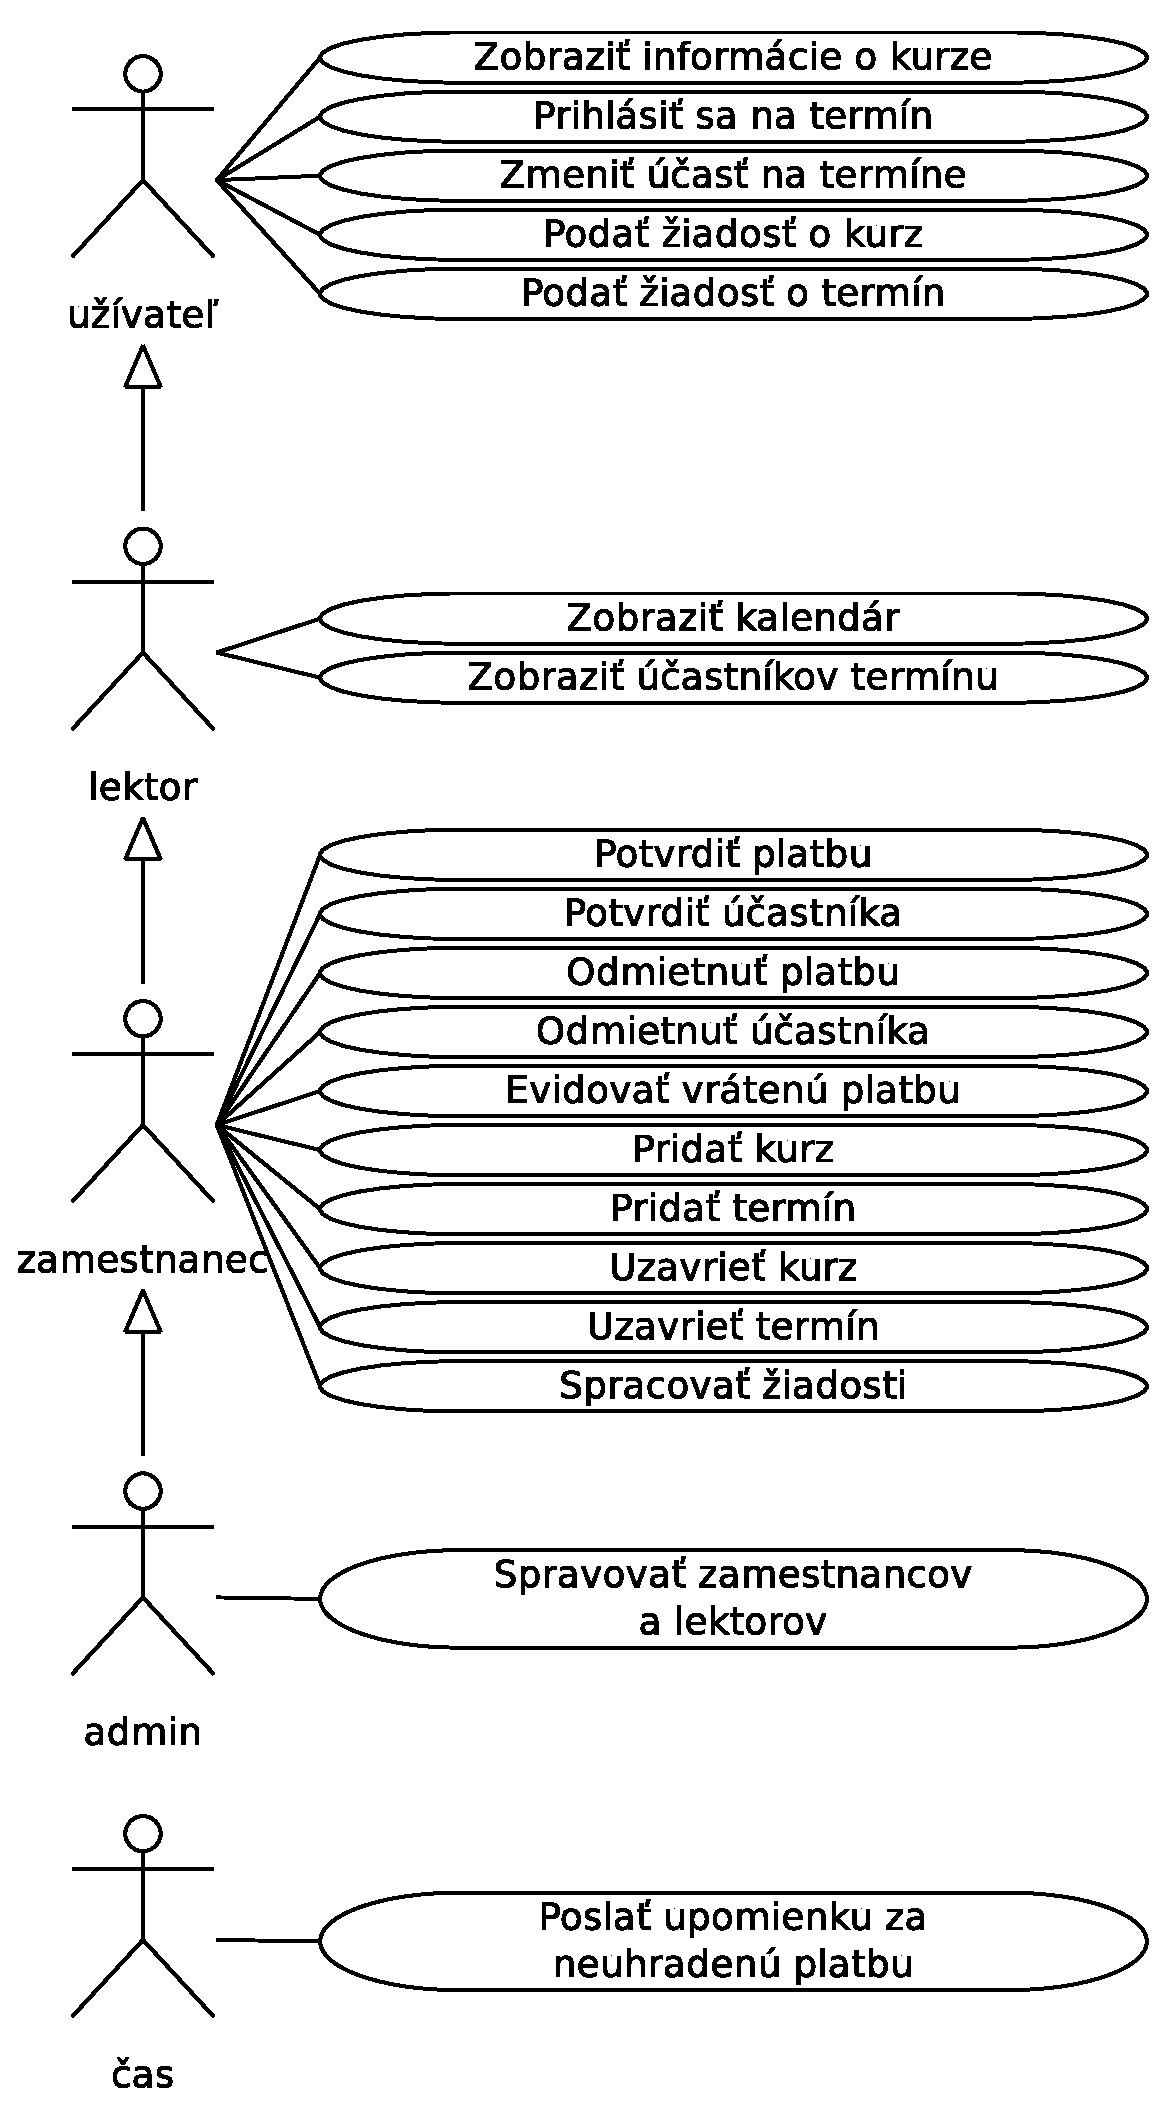
\includegraphics[height=14cm]{img/use_case.eps}
			\captionof{figure}{Kompletní diagram případů použití.}
		\end{center}
		
	\subsection{Plán projektu}
	
Na základě analýzy projektu jsme se rozhodli rozdělit projekt na 4 iterace. V prvních 2 se vytvoří prototypy obsahující drtivou většinu funkcí celého systému. Následně ve 3. iteraci se projekt překlopí již na konečnou implementaci a ve 4. se budou dodělávat funkčnosti usnadňující práci se systémem a zvyšující jeho přehlednost.
	
Prototypování po prvních 2 iteracích nám umožní zhodnotit použitelnost systému dříve, než začne být implementována ostrá verze a pomůže ve shodě se zákazníkem.
	
	\subsubsection{1. iterácia}
		\begin{center}
			\captionsetup{type=figure}
			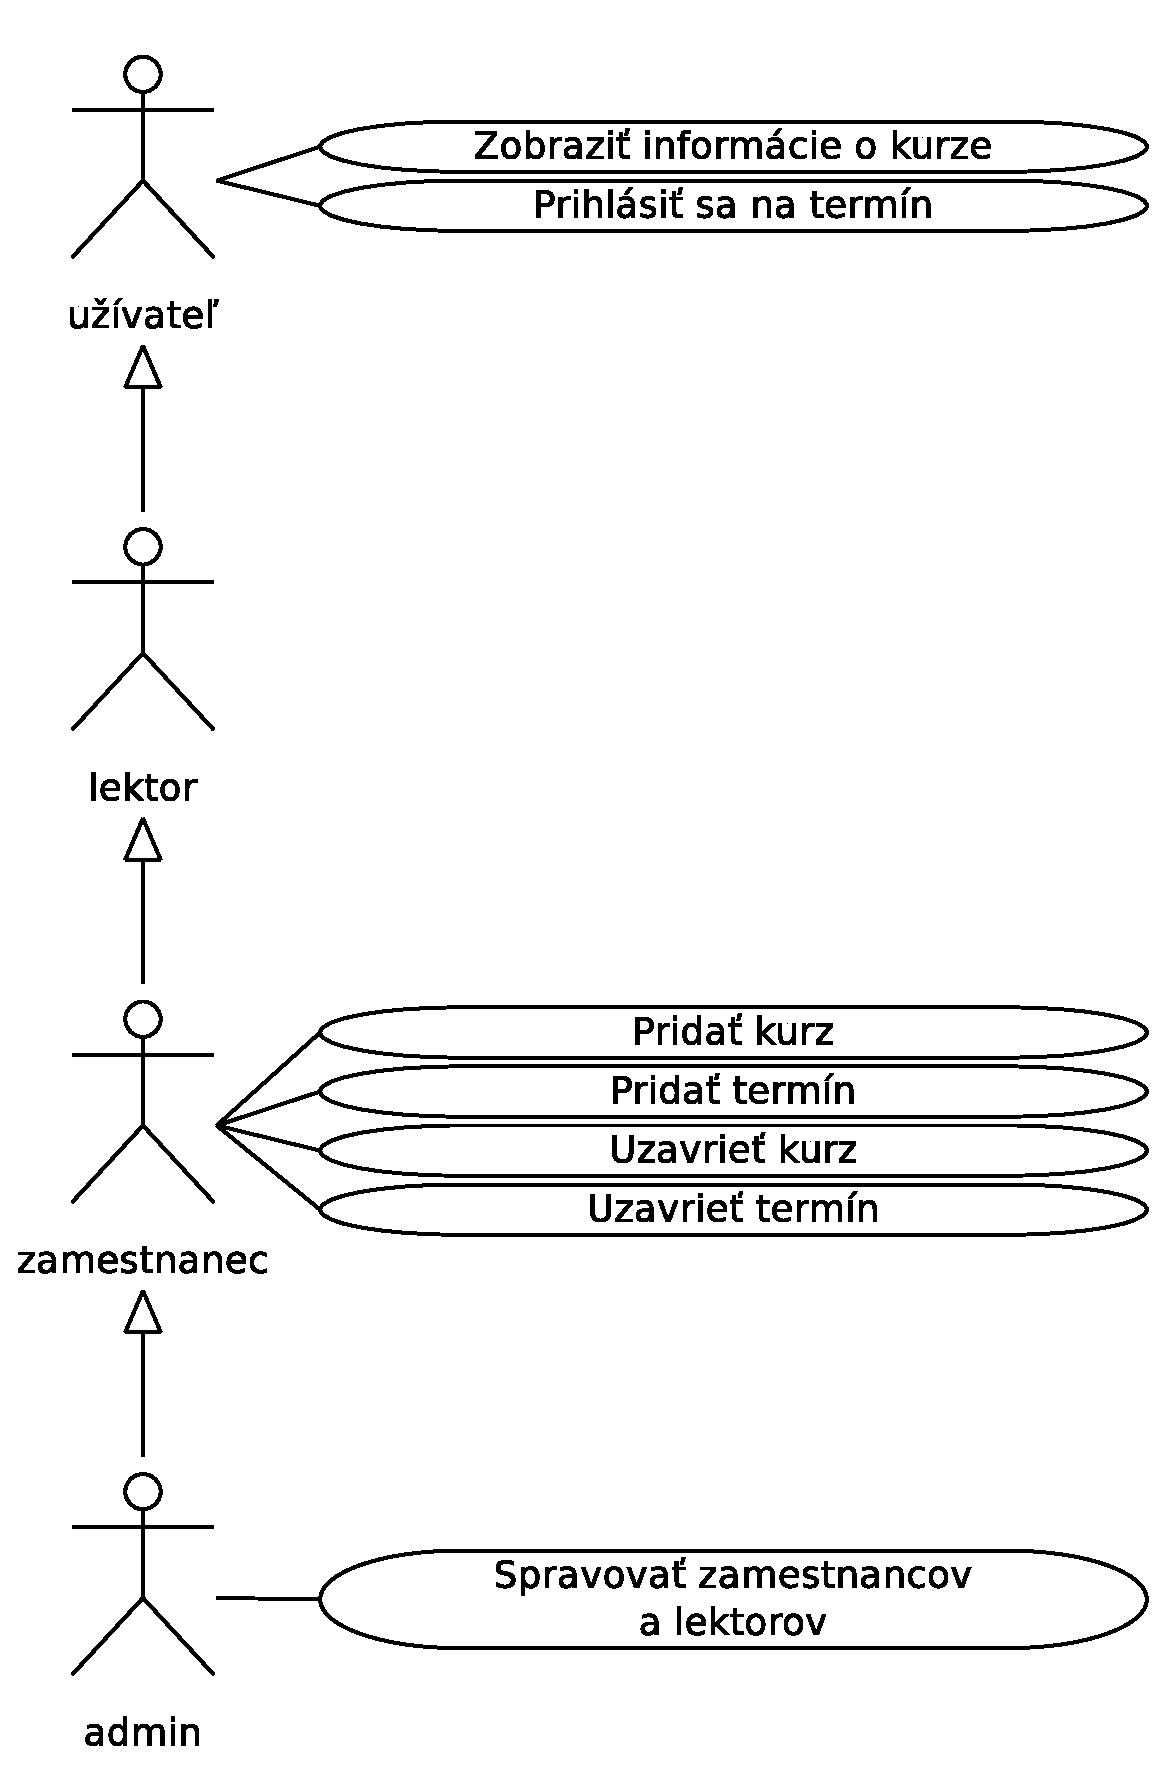
\includegraphics[height=17cm]{img/use_case_iter1.eps}
			\captionof{figure}{Diagram implementovaných případů použití po 1. iteraci.}
		\end{center}
		
Prototyp aplikace bude umět základní správu kurzů a termínů - přidávat a uzavírat kurzy a termíny. Zároveň bude umět přidávat přihlášky a vytvářet uživatele.
	
	\subsubsection{2. iterácia}
		\begin{center}
			\captionsetup{type=figure}
			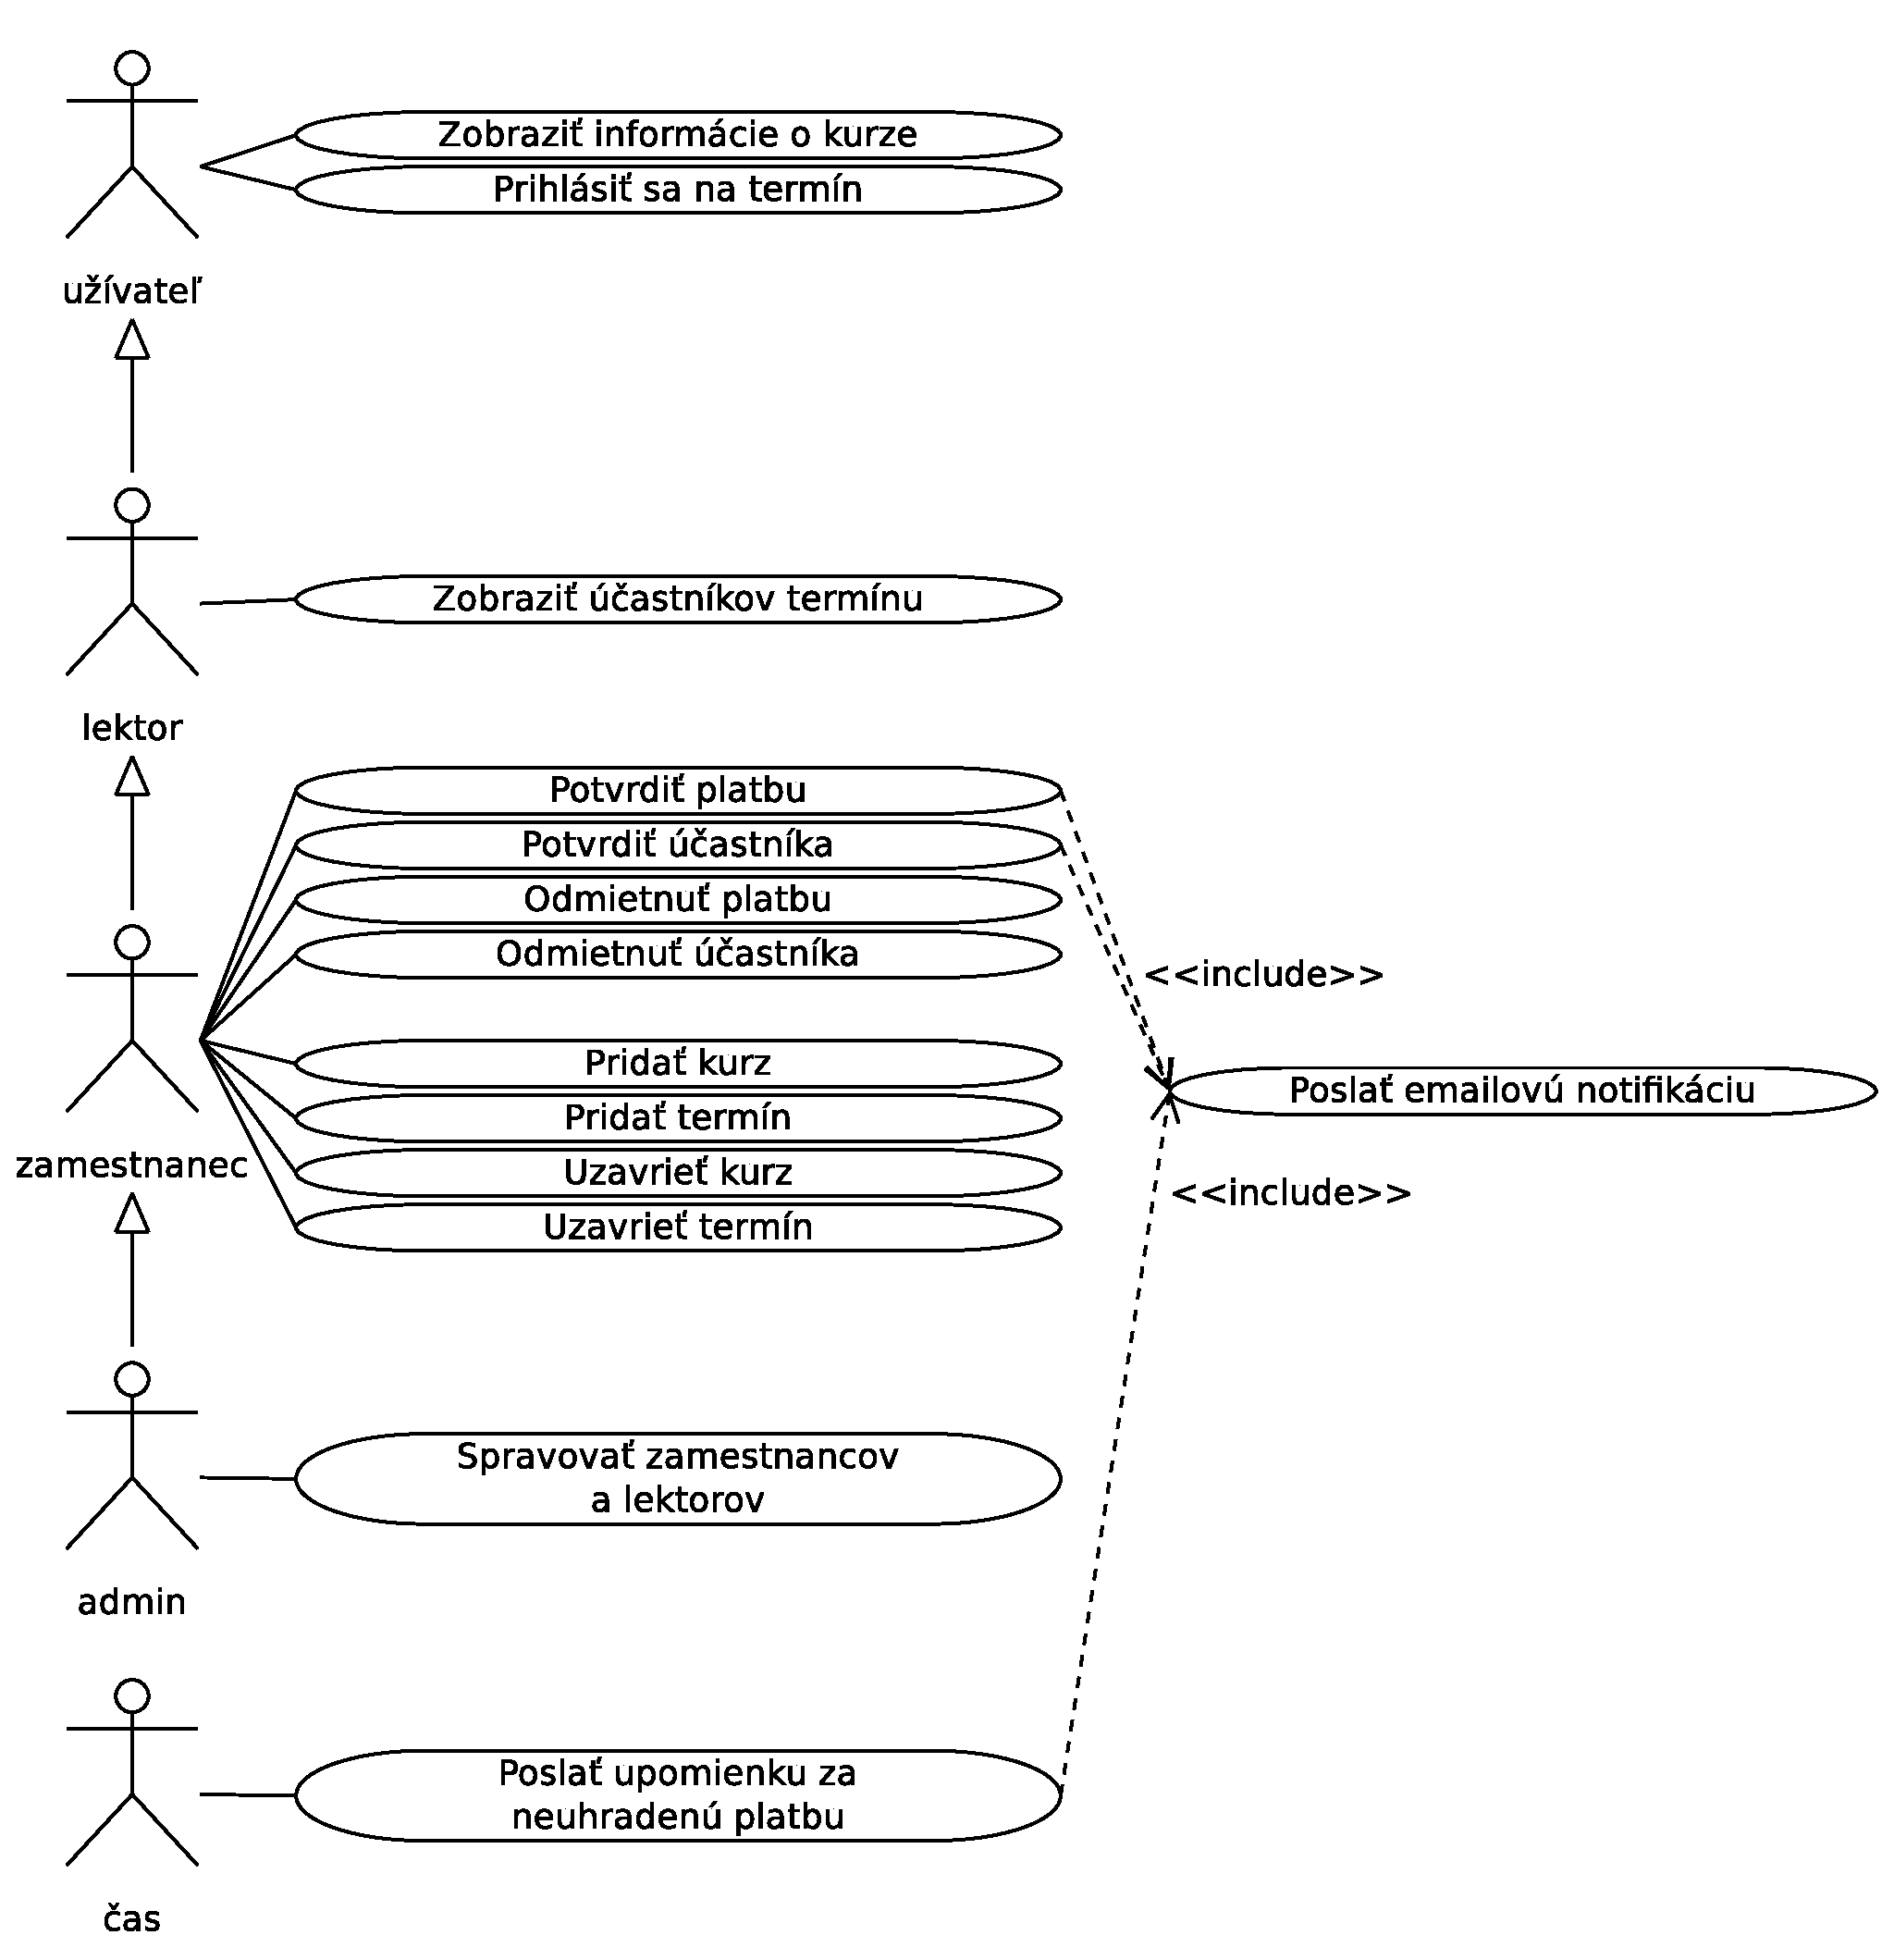
\includegraphics[height=17cm]{img/use_case_iter2.eps}
			\captionof{figure}{Diagram implementovaných případů použití po 2. iteraci.}
		\end{center}			
Ve 2. iteraci se přidá většina zbývajících hlavních funkcí systému. Po přihlášení na kurz bude prototyp již umožňovat potvrdit/odmítnout platbu nebo přihlášku a posílat notifikace nebo upomínky.
	
	\subsubsection{3. iterácia}
		\begin{center}
			\captionsetup{type=figure}
			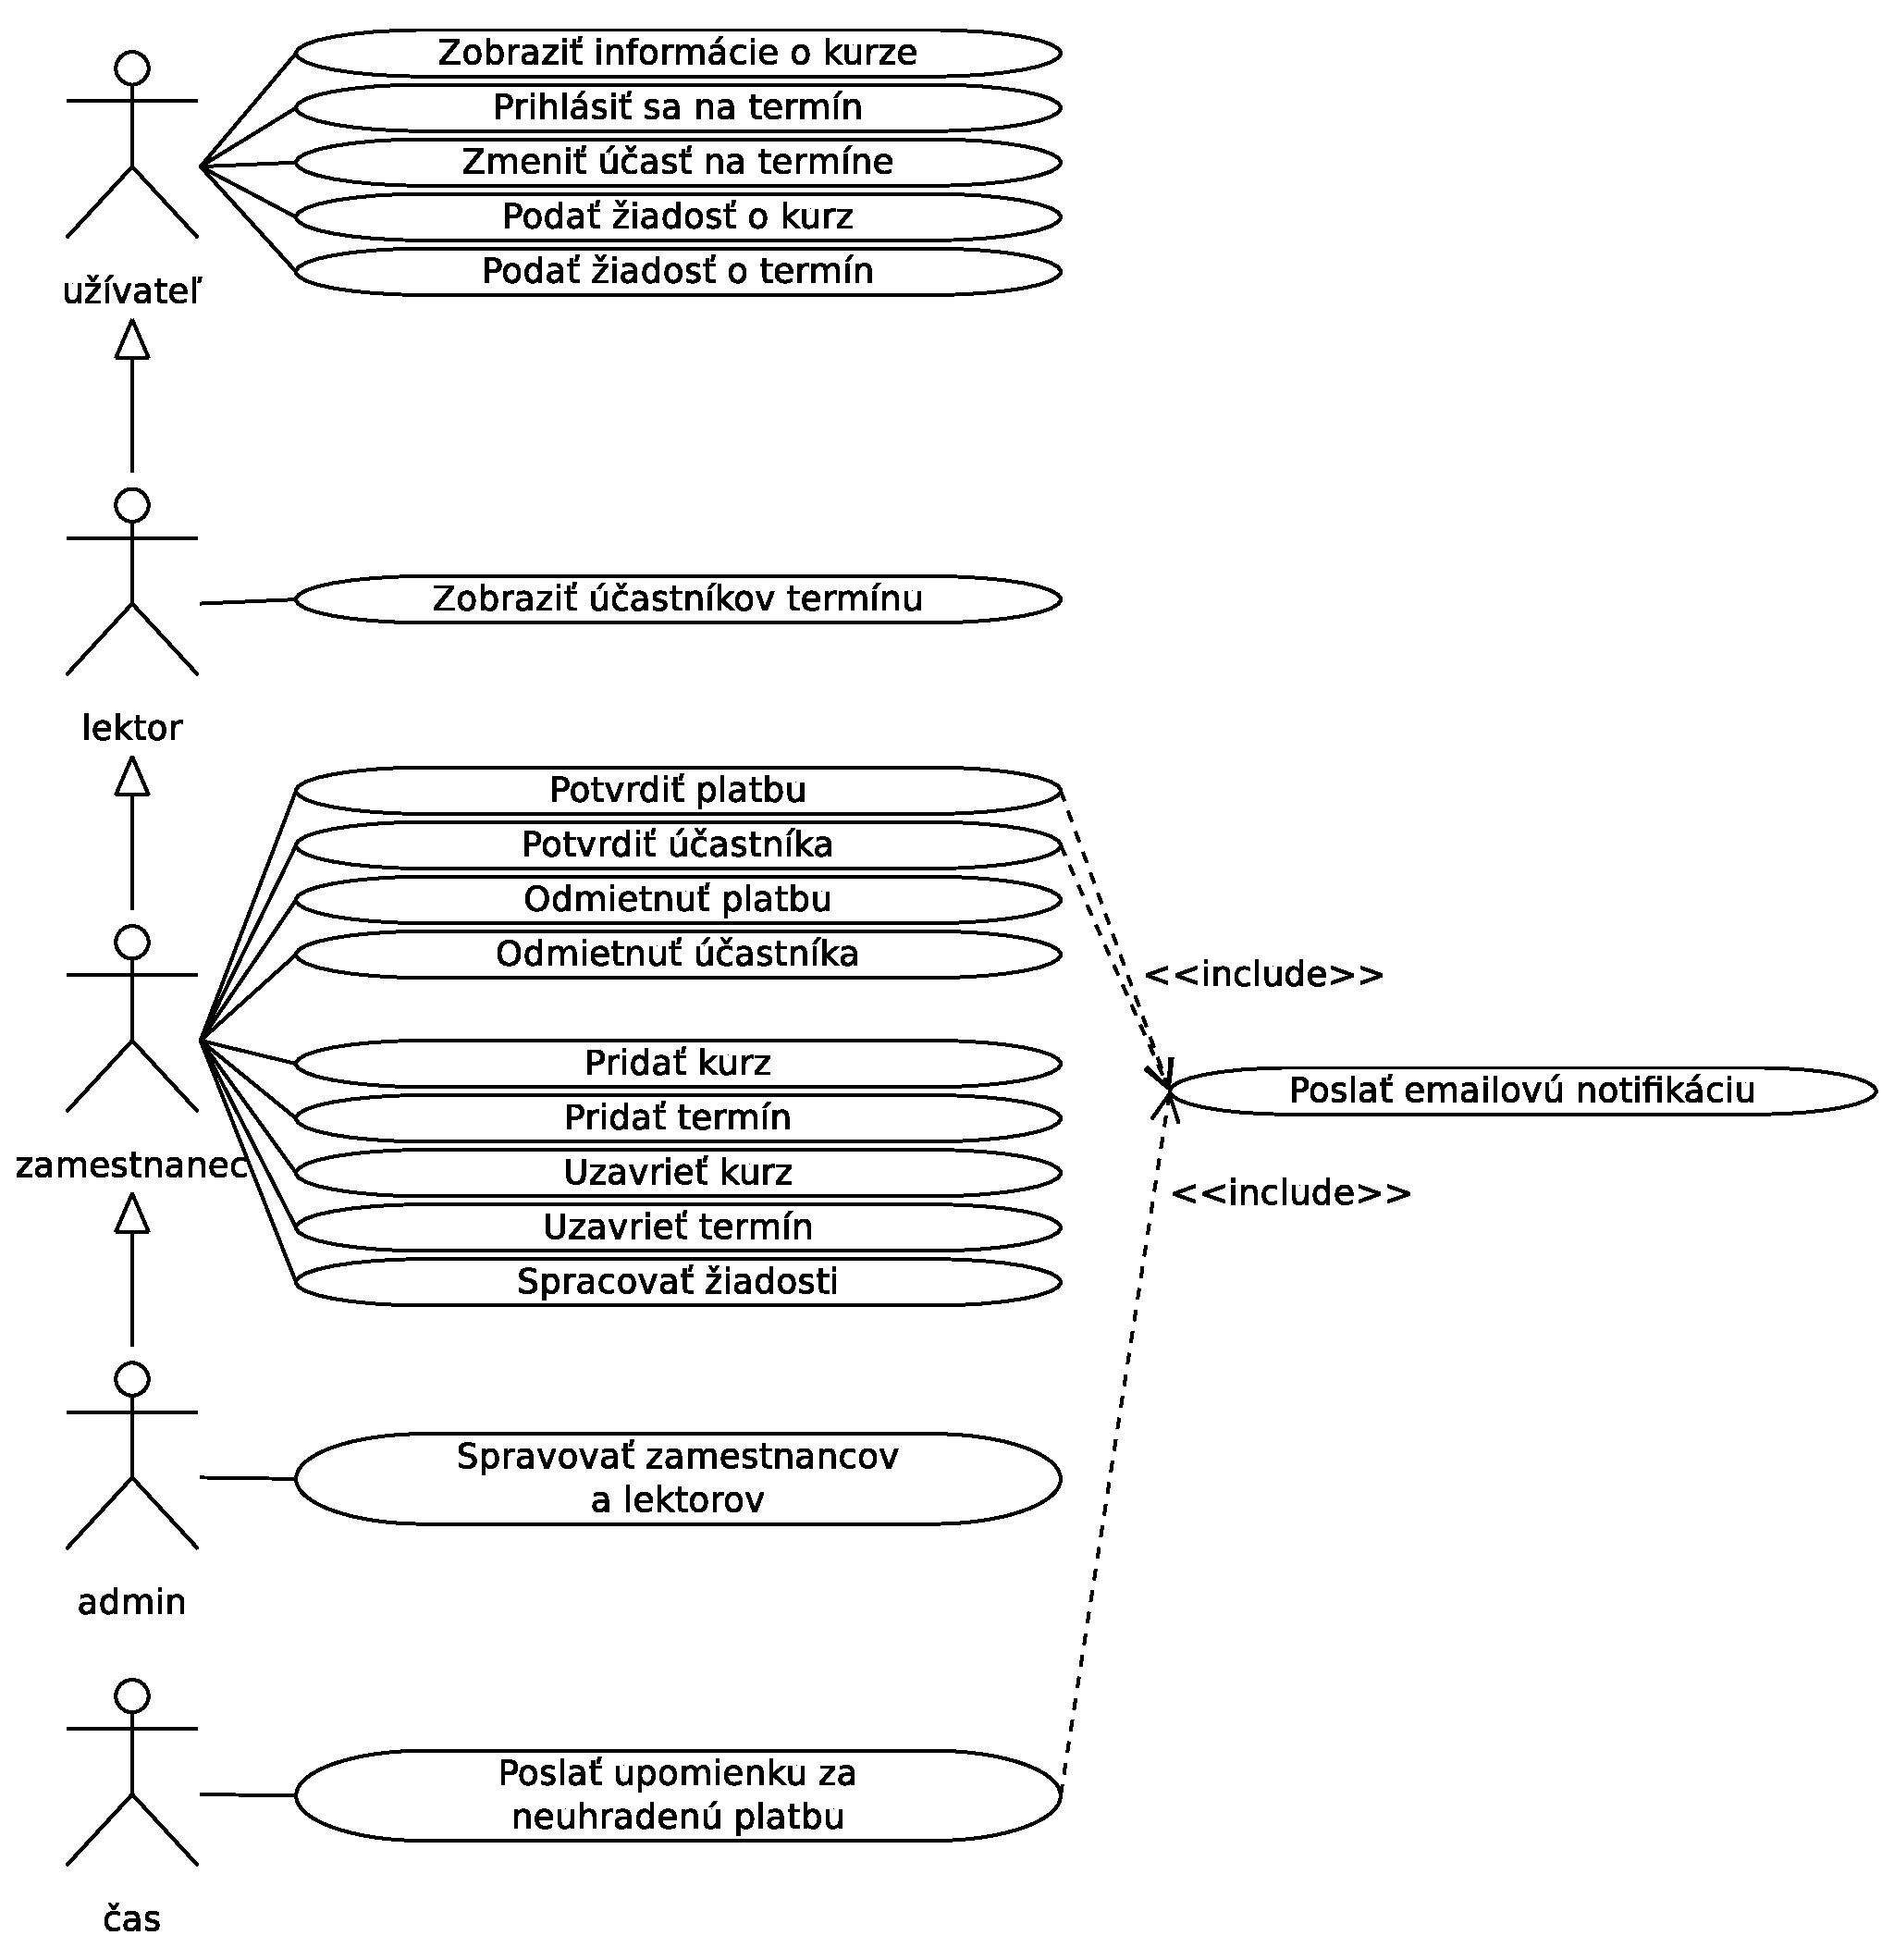
\includegraphics[height=17cm]{img/use_case_iter3.eps}
			\captionof{figure}{Diagram implementovaných případů použití po 3. iteraci.}
		\end{center}
		
Ve 3. iteraci by měl být zákazník spokojený s celkovou funkčností prototypu a ten se začne překlápět na již konečnou implementaci. Zároveň je přidána možnost žádosti o vypsání kursu/termínu a správy vlastní přihlášky.
	
	\subsubsection{4. iterácia}
		\begin{center}
			\captionsetup{type=figure}
			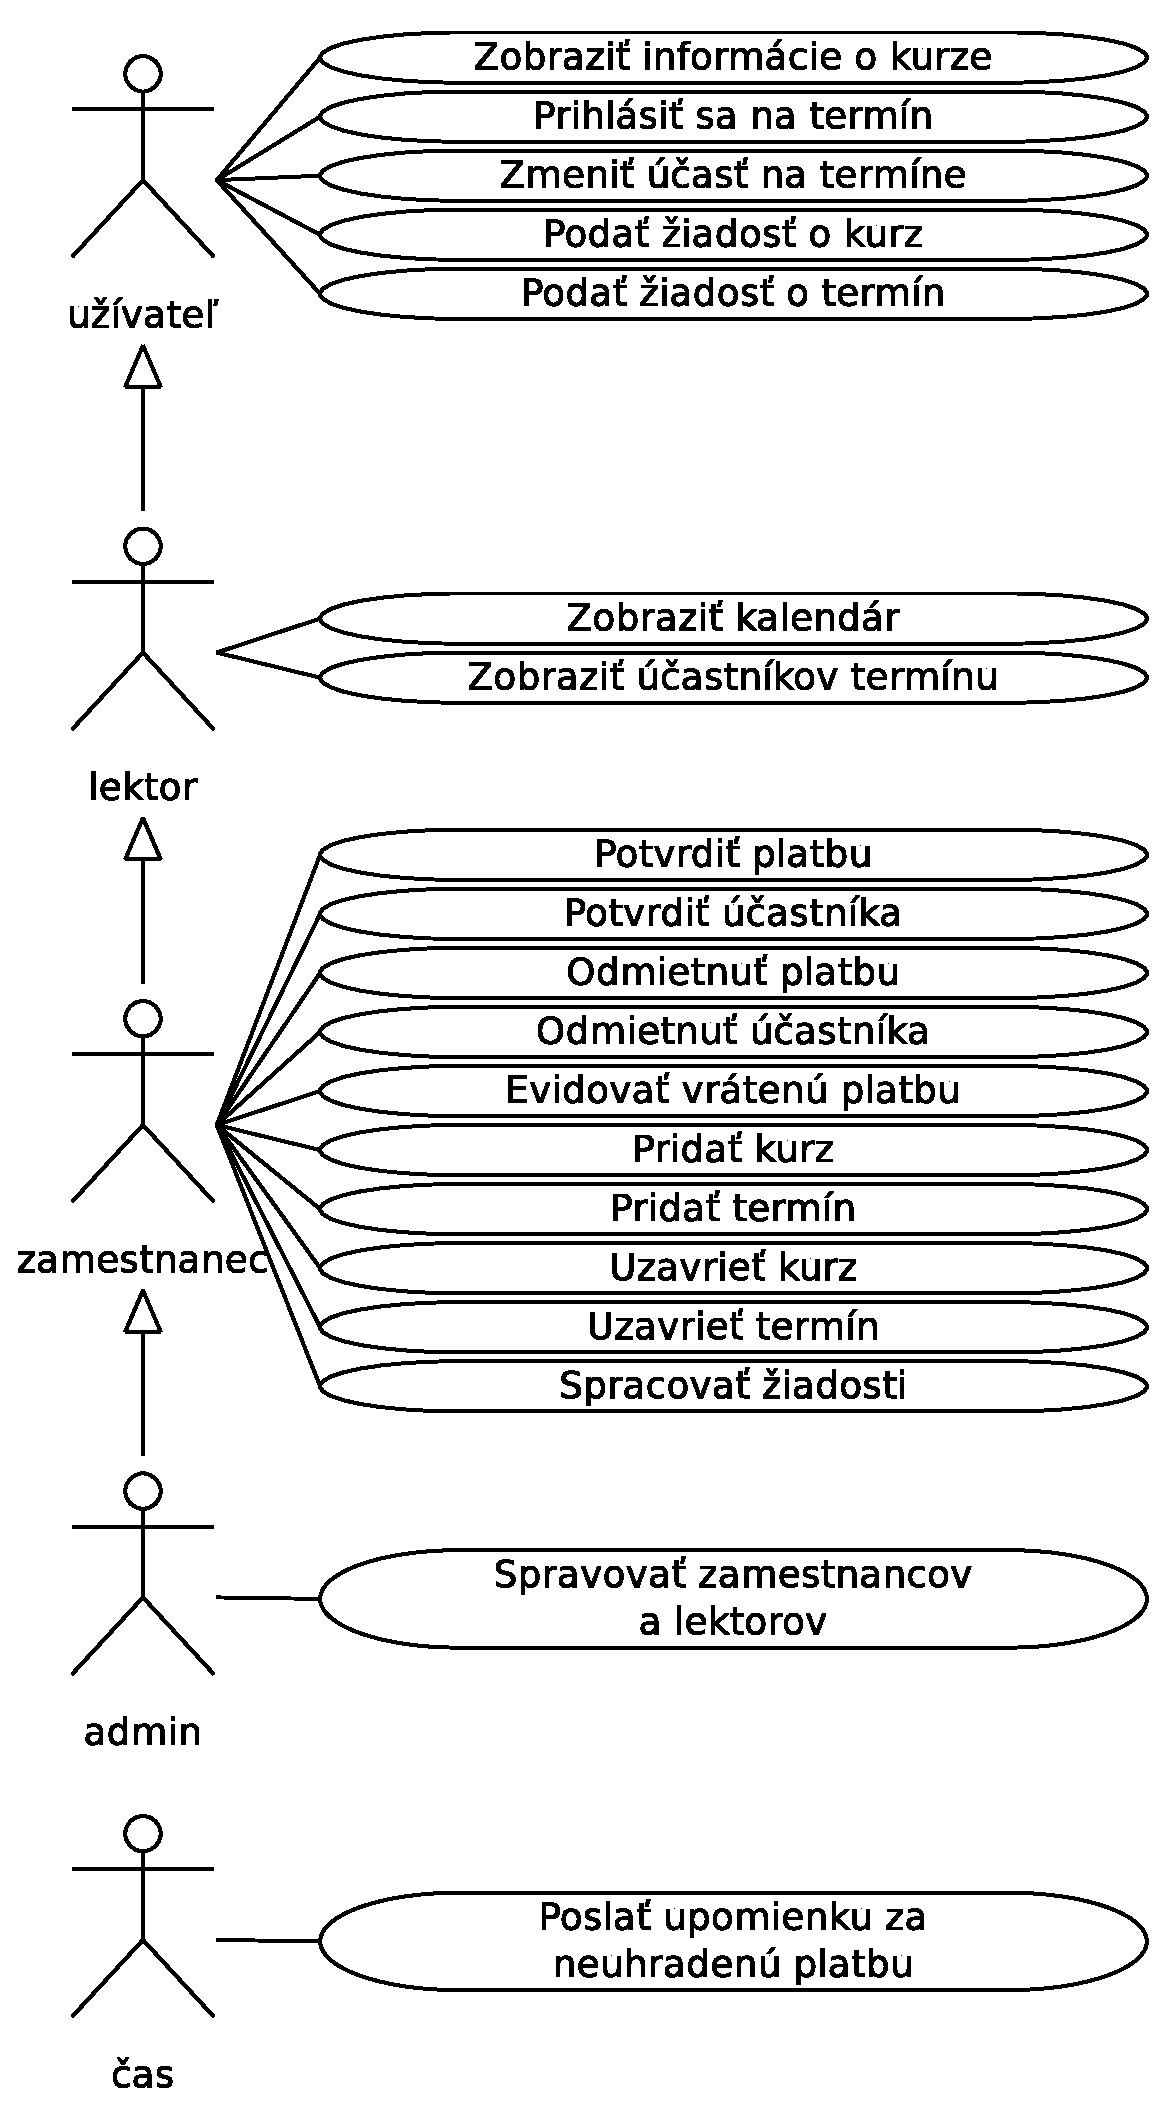
\includegraphics[height=17cm]{img/use_case.eps}
			\captionof{figure}{Diagram implementovaných případů použití po 4. iteraci.}
		\end{center}
		
Ve 4. iteraci se implementuje kalendář a evidence vrácených plateb. Jedná se především o detaily usnadňující práci se systémem, nikoliv už samotnou funkčnost.





%------------------- 1. ITERACE ---------------------%




\chapter{Specifikace}

\section{Specifikace případů použití}

\subsection{Přidat termín}

\begin{center}
    \begin{tabular}{ | p{4.5cm} | p{13cm} | }
    \hline
    \textbf{Název} & Přidat termín 
    \\ \hline
    
	\textbf{Vytvořeno} & Pavel Macenauer 
	\\ \hline
	
	\textbf{Popis} & Ke kurzu se vytvoří termín, tj. časový rozsah, kdy bude probíhat výuka daného kurzu. 
	\\ \hline
	    
	\textbf{Primární aktéři} & Zaměstnanec
	\\ \hline
	
	\textbf{Sekundární aktéři} & Admin		   
	\\ \hline
	
	\textbf{Předpoklady} & Vybrán existující kurz
    \\ \hline
    
    \textbf{Následné podmínky} & Přidán termín ke kurzu
    \\ \hline 
        
    \textbf{Akce pro spuštění} & Zaměstnanec klikne na tlačítko "Přidat termín" u konkrétního kurzu.
    \\ \hline
    
    \textbf{Hlavní tok} & 1. Zaměstnanec vybere konkrétní kurz 
    	\newline 2. Zaměstnanec klikne na "Přidat termín" 
    	\newline 3. Zaměstnanec vyplní formulář a klikne na "Přidat" 
    	\newline 4. Systém zpracuje formulář a přidá nový termín
    \\ \hline
    
    \textbf{Alternativní toky} & -
    \\ \hline -
    
    \textbf{Vyjímky} & 1. Chybný vstup
    	\newline 2. Obsazený lektor
    \\ \hline
    
	\textbf{Frekvence} & Několikrát za týden
	\\ \hline
	
	\textbf{Speciální požadavky} & -
	\\ \hline
    
    
    \end{tabular}
\end{center}
	
	


\end{document}
